% !TEX TS-program = pdflatex
% !TEX encoding = UTF-8 Unicode

\documentclass{beamer}
% for handouts: \documentclass[handout]{beamer}

%\setbeamertemplate{background canvas}[vertical shading][bottom=white,top=structure.fg!25]
% or whatever

\usetheme[compress]{Amsterdam}
%\setbeamertemplate{headline}{}
%\setbeamertemplate{footline}{}
%\setbeamersize{text margin left=0.5cm}
  
\usepackage[english]{babel}
\usepackage{listings}
\usepackage{geometry}
\usepackage{hyperref}

\usepackage{color}
\usepackage[T1]{fontenc}
\usepackage[utf8]{inputenc}
\usepackage{lmodern}

\usepackage{multicol}
\lstset{
basicstyle=\scriptsize\ttfamily,
columns=flexible,
breaklines=true,
numbers=left,
%stepsize=1,
numberstyle=\tiny,
backgroundcolor=\color[rgb]{0.85,0.90,1}
}


\begin{document}

\title{Unsupervised approaches to detecting topics in news and politics}
\author[Damian Trilling]{Damian Trilling \\ ~ \\ \footnotesize{d.c.trilling@uva.nl \\@damian0604} \\ \url{www.damiantrilling.net}}
\date[18 October 2019]{18 October 2019, Salamanca}
\institute[UvA]{Afdeling Communicatiewetenschap \\Universiteit van Amsterdam}


\begin{frame}{}
\titlepage
\end{frame}

\begin{frame}{Today}
\tableofcontents
\end{frame}




\section{Types of Automated Content Analysis}
\begin{frame}{}
Types of Automated Content Analysis
\end{frame}
\subsection*{Top-down vs. bottom-up}


%{\setbeamercolor{background canvas}{bg=black}
\begin{frame}[plain]
\makebox[\linewidth]{
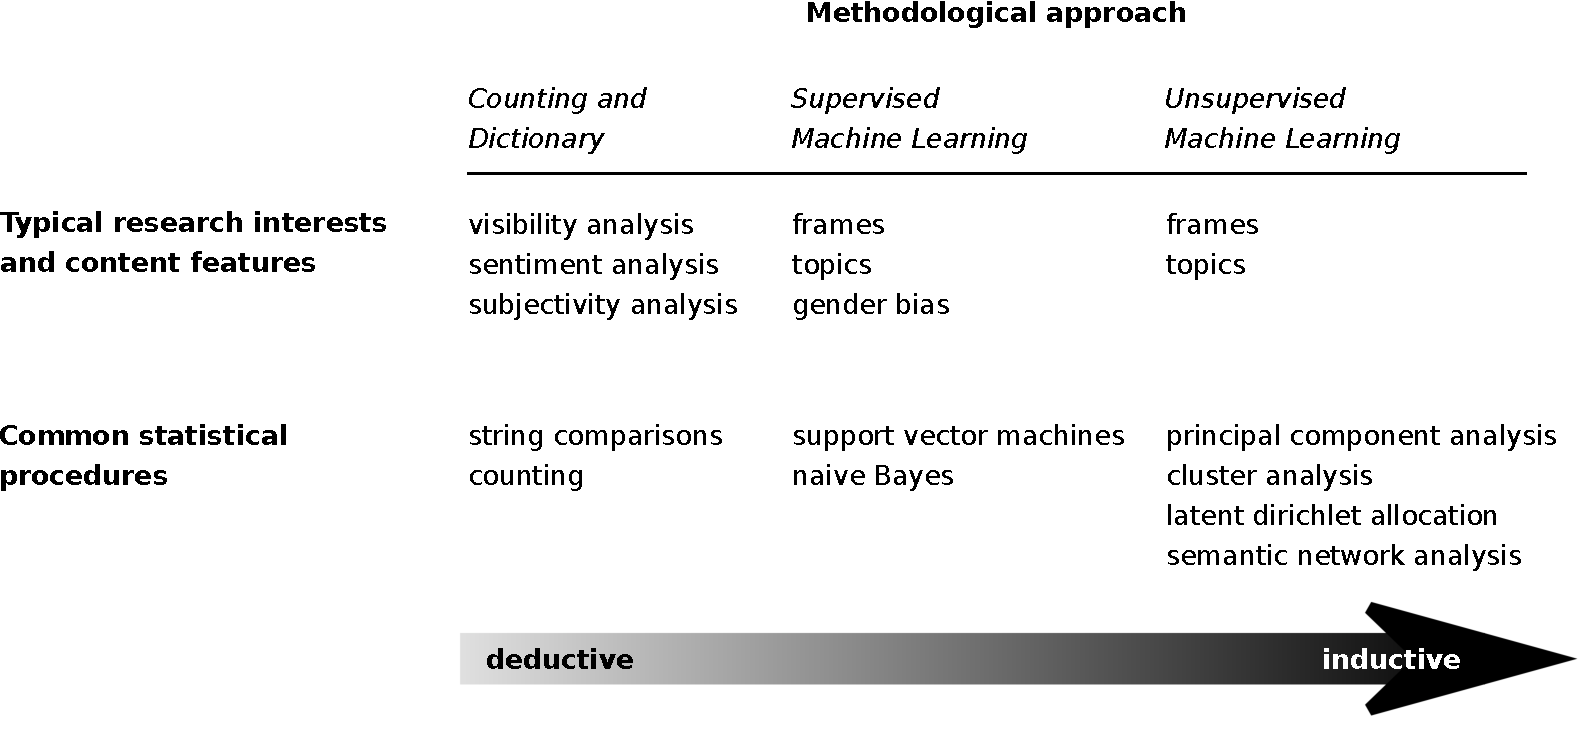
\includegraphics[width=\paperwidth,height=\paperheight,keepaspectratio]{../pictures/boumanstrilling2016}}

\tiny{Boumans, J. W., \& Trilling, D. (2016). Taking stock of the toolkit: An overview of relevant autmated content analysis approaches and techniques for digital journalism scholars. \textit{Digital Journalism, 4}(1), 8–23. doi:10.1080/21670811.2015.1096598}
\end{frame}
%}




\begin{frame}{Some terminology }
\begin{columns}[t]
\column{.5\textwidth}

\begin{block}<1-4>{Supervised machine learning}
You have a dataset with both predictor and outcome (independent and dependent variables; features and labels) --- a \emph{labeled} dataset.
\onslide<2>{
	\footnotesize{Think of regression: You measured \texttt{x1}, \texttt{x2}, \texttt{x3} and you want to predict \texttt{y}, which you also measured}}
\end{block}

\column{.5\textwidth}

\begin{block}<3->{Unsupervised machine learning}
You have no labels. \onslide<4>{(\footnotesize{You did not measure \texttt{y})}}\\
\onslide<5>{\textbf{You probably already know some techniques to find out how \texttt{x1}, \texttt{x2},\ldots \texttt{x\_i} co-occur:} \begin{itemize}
		\item Principal Component Analysis (PCA) and Singular Value Decomposition (SVD)
		\item Cluster analysis
		%\item Topic modelling (Non-negative matrix factorization and Latent Dirichlet Allocation)
		\item \ldots
	\end{itemize}
}
\end{block}

\end{columns}

\end{frame}


\section[PCA and Clustering]{PCA and Clustering}
\begin{frame}{}
PCA and Clustering
\end{frame}
\subsection*{PCA and Clustering}


\begin{frame}{Let's assume we want to find out the topics in a large corpus of documents}
We could, for example
\begin{itemize}
	\item use PCA to find out related features (and interpret those as topics)
	\item or use clustering to find similar documents (and then look at the words they share to interpret as topics)
\end{itemize}

\pause

Actually, we have \emph{two} things we want to model:

\begin{enumerate}
	\item Which topics can we extract from the corpus?
	\item How present is each of these topics in each text in the corpus?
\end{enumerate}

\end{frame}


\begin{frame}[fragile]{Recap: PCA}
Document-term matrix
\begin{lstlisting}
       w1,w2,w3,w4,w5,w6 ...
text1, 2, 0, 0, 1, 2, 3 ...
text2, 0, 0, 1, 2, 3, 4 ...
text3, 9, 0, 1, 1, 0, 0 ...
...
\end{lstlisting}
{\small{These can be simple counts, but also more advanced metrics, like tf-idf scores (where you weigh the frequency by the number of documents in which it occurs), cosine distances, etc.}}
\pause
	\begin{itemize}
	\item given a term-document matrix, easy to do with any tool
	\item probably extremely skewed distributions
	\item some problematic assumptions: \textcolor{red}{does the goal of PCA, to find a solution in which one word loads on \emph{one} component match real life, where a word can belong to several topics or frames?}
\end{itemize}

\end{frame}


\begin{frame}{Recap: clustering}
\begin{itemize}
	\item given a term-document matrix, we can easily find clusters of documents that resemble each other
	\item but also here \textcolor{red}{does the goal of cluster analysis, assigning each document to \emph{one} cluster, match real life?}
\end{itemize}
\end{frame}


\begin{frame}{We need other models to}
\begin{enumerate}[<+->]
	\item model \emph{simultaneously} (a) which topics we find in the whole corpus, and (b) which of these topics are present in which document; while at the same time
	\item allowing (a) words to be part of multiple topics, and (b) multiple topics to be present in one document; and
	\item being able to make connections between words ``even if they never actually occured in a document together'' (Maier et al, 2018, p.~96)
\end{enumerate}

\tiny{Maier, D., Waldherr, A., Miltner, P., Wiedemann, G., Niekler, A., Keinert, A., \ldots Adam, S. (2018). Applying LDA Topic Modeling in Communication Research: Toward a Valid and Reliable Methodology. \textit{Communication Methods and Measures, 12}(2--3), 93--118. doi:10.1080/19312458.2018.1430754}
\end{frame}



\section{LDA Topic models}

\subsection{An introduction to LDA}

\begin{frame}{}
	Enter \textbf{topic modeling with Latent Dirichlet Allocation (LDA)}
\end{frame}






\begin{frame}{LDA, what's that?}
	\begin{block}{No mathematical details here, but the general idea}
		\begin{itemize}
			\item There are $k$ topics, $T_1$\ldots$T_k$
			\item Each document $D_i$ consists of a mixture of these topics, e.g.$80\% T_1, 15\% T_2, 0\% T_3, \ldots 5\% T_k $
			\item On the next level, each topic consists of a specific probability distribution of words
			\item Thus, based on the frequencies of words in $D_i$, one can infer its distribution of topics
			\item Note that LDA (like PCA) is a Bag-of-Words (BOW) approach
		\end{itemize}
	\end{block}
	
\end{frame}




\begin{frame}[fragile]{Doing a LDA in Python}
You can use gensim ({\v R}eh{\r u}{\v r}ek \& Sojka, 2010) for this.

Let us assume you have a list of lists of words (!) called \texttt{texts}:

\begin{lstlisting}
articles=['The tax deficit is higher than expected. This said xxx ...', 'Germany won the World Cup. After a']
texts=[art.split() for art in articles]
\end{lstlisting}
which looks like this:
\begin{lstlisting}
[['The', 'tax', 'deficit', 'is', 'higher', 'than', 'expected.', 'This', 'said', 'xxx', '...'], ['Germany', 'won', 'the', 'World', 'Cup.', 'After', 'a']]
\end{lstlisting}

\tiny{{\v R}eh{\r u}{\v r}ek, R., \& Sojka, P. (2010). Software framework for topic modelling with large corpora. \emph{Proceedings of the LREC 2010 Workshop on New Challenges for NLP Frameworks}, pp. 45–50. Valletta, Malta: ELRA. }

\end{frame}




\begin{frame}[plain,fragile]
\begin{lstlisting}
from gensim import corpora, models

NTOPICS = 100
LDAOUTPUTFILE="topicscores.tsv"

# Create a BOW represenation of the texts
id2word = corpora.Dictionary(texts)
mm =[id2word.doc2bow(text) for text in texts]

# Train the LDA models.
mylda = models.ldamodel.LdaModel(corpus=mm, id2word=id2word, num_topics=NTOPICS, alpha="auto")

# Print the topics.
for top in mylda.print_topics(num_topics=NTOPICS, num_words=5):
  print ("\n",top)

print ("\nFor further analysis, a dataset with the topic score for each document is saved to",LDAOUTPUTFILE)

scoresperdoc=mylda.inference(mm)

with open(LDAOUTPUTFILE,"w",encoding="utf-8") as fo:
  for row in scoresperdoc[0]:
    fo.write("\t".join(["{:0.3f}".format(score) for score in row]))
fo.write("\n")
\end{lstlisting}

\end{frame}


\begin{frame}[fragile]{Output: Topics (below) \& topic scores (next slide)}
\begin{lstlisting}
0.069*fusie + 0.058*brussel + 0.045*europesecommissie + 0.036*europese + 0.023*overname
0.109*bank + 0.066*britse + 0.041*regering + 0.035*financien + 0.033*minister
0.114*nederlandse + 0.106*nederland + 0.070*bedrijven + 0.042*rusland + 0.038*russische
0.093*nederlandsespoorwegen + 0.074*den + 0.036*jaar + 0.029*onderzoek + 0.027*raad
0.099*banen + 0.045*jaar + 0.045*productie + 0.036*ton + 0.029*aantal
0.041*grote + 0.038*bedrijven + 0.027*ondernemers + 0.023*goed + 0.015*jaar
0.108*werknemers + 0.037*jongeren + 0.035*werkgevers + 0.029*jaar + 0.025*werk
0.171*bank + 0.122* + 0.041*klanten + 0.035*verzekeraar + 0.028*euro
0.162*banken + 0.055*bank + 0.039*centrale + 0.027*leningen + 0.024*financiele
0.052*post + 0.042*media + 0.038*nieuwe + 0.034*netwerk + 0.025*personeel
...
\end{lstlisting}
\end{frame}


\begin{frame}[plain]
\makebox[\linewidth]{
	\includegraphics[width=\paperwidth,height=\paperheight,keepaspectratio]{../pictures/topicscores}}
\end{frame}




\begin{frame}[fragile]{Visualization with pyldavis}
\begin{lstlisting}
import pyLDAvis
import pyLDAvis.gensim
# first estiate gensim model, then:
vis_data = pyLDAvis.gensim.prepare(mylda,mm,id2word)
pyLDAvis.display(vis_data)
\end{lstlisting}
\makebox[\linewidth]{
	\includegraphics[width=\paperwidth,height=.5\paperheight,keepaspectratio]{../pictures/pyldavis}}
\end{frame}

\begin{frame}{Visualization with pyldavis}
Short note about the $\lambda$ setting:

It influences the ordering of the words in pyldavis.

\begin{quote}
``For $\lambda = 1$, the ordering of the top words is equal to the ordering of the standard conditional word probabilities. For $\lambda$ close to zero, the most specific words of the topic will lead the list of top words. In their case study, Sievert and Shirley (2014, p. 67) found the best interpretability of topics using a  $\lambda$-value close to .6, which we adopted for our own case'' (Maier et al., 2018, p.~107)
\end{quote}


\tiny{Maier, D., Waldherr, A., Miltner, P., Wiedemann, G., Niekler, A., Keinert, A., \ldots Adam, S. (2018). Applying LDA Topic Modeling in Communication Research: Toward a Valid and Reliable Methodology. \textit{Communication Methods and Measures, 12}(2--3), 93--118. doi:10.1080/19312458.2018.1430754}
\end{frame}


%\begin{frame}[plain]{Code examples}
%\url{https://github.com/damian0604/bdaca/blob/master/rm-course-2/week12/lda.ipynb}
%\end{frame}



\subsection{Choosing the best (or a good) topic model}

\begin{frame}{Choosing the best (or a good) topic model}
\begin{itemize}
	\item There is no single best solution (e.g., do you want more coarse or fine-grained topics?)
	\item Non-deterministic
	\item Very sensitive to preprocessing choices
	\item Interplay of both metrics and (qualitative) interpretability 
\end{itemize}

See for more elaborate guidance:

\tiny{Maier, D., Waldherr, A., Miltner, P., Wiedemann, G., Niekler, A., Keinert, A., \ldots Adam, S. (2018). Applying LDA Topic Modeling in Communication Research: Toward a Valid and Reliable Methodology. \textit{Communication Methods and Measures, 12}(2--3), 93--118. doi:10.1080/19312458.2018.1430754}

\end{frame}



\begin{frame}{Evaluation metrics (closer to zero is better)}
\begin{block}{perplexity}
A goodness-of-fit measure, answering the question: If we do a train-test split, how well does the trained model fit the test data?
\end{block}

\pause 
\begin{block}{coherence}
\begin{itemize}
\item mean coherence of the whole model: attempts to quantify the interpretability
\item coherence per topic: allows to get topics that are most likely to be coherently interpreted (\texttt{.top\_topics()})
\end{itemize}
\end{block}

\end{frame}



\begin{frame}{Choosing $k$: How many topics do we want?}
\begin{itemize}
	\item Typical values: $10<k<200$
	\item Too low: losing nuance, so broad it becomes meaningless
	\item Too high: picks up tiny pecularities instead of finding general patterns
	\item There is no inherent ordering of topics (unlike PCA!)
	\item We can throw away or merge topics later, so if out of $k=50$ topics 5 are not interpretable and a couple of others overlap, it still may be a good model
\end{itemize}
\end{frame}


\begin{frame}[fragile]{Choosing $\alpha$: how sparse should the document-topic distribution $\theta$ be?}
\begin{itemize}
	\item The higher $\alpha$, the more topics per document 
	\item Default: $1/k$
	\item But: We can explicitly change it, or -- really cool -- even learn $\alpha$ from the data (\texttt{alpha = "auto"})
\end{itemize}

\pause 

Takeaway: It takes longer, but you probably want to learn alpha from the data, using multiple passes:

\begin{lstlisting}
mylda LdaModel(corpus=tfidfcorpus[ldacorpus], id2word=id2word, num_topics=50, alpha='auto', passes=10)
\end{lstlisting}


\end{frame}


\begin{frame}{Choosing $\eta$: how sparse should the topic-word distribution $\lambda$ be?}
\begin{itemize}
	\item Can be used to boost specific words
	\item Can also be learned from the data 
\end{itemize}

\pause
Takeaway: Even though you can do \texttt{eta="auto"}, this usually does not help you much.

\end{frame}


% \subsection{Drawbacks of LDA topic models}


\subsection{Using topic models}

\begin{frame}{Using topic models}

You got your model -- what now?

\begin{enumerate}
	\item Assign topic scores to documents
	\item Label topics
	\item Merge topics, throw away boilerplate topics and similar (manually, or aided by cluster analysis)
	\item Compare topics between, e.g., outlets
	\item or do some time-series analysis.
\end{enumerate}


Example:
\tiny{Tsur, O., Calacci, D., \& Lazer, D. (2015). A Frame of Mind: Using Statistical Models for Detection of Framing and Agenda Setting Campaigns. \textit{Proceedings of the 53rd Annual Meeting of the Association for Computational Linguistics and the 7th International Joint Conference on Natural Language Processing} (pp. 1629–1638).}



\end{frame}



\subsection{Other forms of topic models}


\begin{frame}[plain]
Other forms of topic models
\end{frame}

\begin{frame}{Other forms of topic models}
\begin{itemize}
	\item Author-topic models
	\item Structural topic models
	\item Non-negative matrix factorization
	\item \ldots
\end{itemize}
\end{frame}




\section{Let's do it!}
\begin{frame}[plain]

\centering
\Huge{Let's do it!}
\vspace{2cm}

\normalsize{(go to Google colab)}
\end{frame}




\end{document}

